% Options for packages loaded elsewhere
\PassOptionsToPackage{unicode}{hyperref}
\PassOptionsToPackage{hyphens}{url}
%
\documentclass[
]{book}
\usepackage{amsmath,amssymb}
\usepackage{lmodern}
\usepackage{iftex}
\ifPDFTeX
  \usepackage[T1]{fontenc}
  \usepackage[utf8]{inputenc}
  \usepackage{textcomp} % provide euro and other symbols
\else % if luatex or xetex
  \usepackage{unicode-math}
  \defaultfontfeatures{Scale=MatchLowercase}
  \defaultfontfeatures[\rmfamily]{Ligatures=TeX,Scale=1}
\fi
% Use upquote if available, for straight quotes in verbatim environments
\IfFileExists{upquote.sty}{\usepackage{upquote}}{}
\IfFileExists{microtype.sty}{% use microtype if available
  \usepackage[]{microtype}
  \UseMicrotypeSet[protrusion]{basicmath} % disable protrusion for tt fonts
}{}
\makeatletter
\@ifundefined{KOMAClassName}{% if non-KOMA class
  \IfFileExists{parskip.sty}{%
    \usepackage{parskip}
  }{% else
    \setlength{\parindent}{0pt}
    \setlength{\parskip}{6pt plus 2pt minus 1pt}}
}{% if KOMA class
  \KOMAoptions{parskip=half}}
\makeatother
\usepackage{xcolor}
\usepackage{longtable,booktabs,array}
\usepackage{calc} % for calculating minipage widths
% Correct order of tables after \paragraph or \subparagraph
\usepackage{etoolbox}
\makeatletter
\patchcmd\longtable{\par}{\if@noskipsec\mbox{}\fi\par}{}{}
\makeatother
% Allow footnotes in longtable head/foot
\IfFileExists{footnotehyper.sty}{\usepackage{footnotehyper}}{\usepackage{footnote}}
\makesavenoteenv{longtable}
\usepackage{graphicx}
\makeatletter
\def\maxwidth{\ifdim\Gin@nat@width>\linewidth\linewidth\else\Gin@nat@width\fi}
\def\maxheight{\ifdim\Gin@nat@height>\textheight\textheight\else\Gin@nat@height\fi}
\makeatother
% Scale images if necessary, so that they will not overflow the page
% margins by default, and it is still possible to overwrite the defaults
% using explicit options in \includegraphics[width, height, ...]{}
\setkeys{Gin}{width=\maxwidth,height=\maxheight,keepaspectratio}
% Set default figure placement to htbp
\makeatletter
\def\fps@figure{htbp}
\makeatother
\setlength{\emergencystretch}{3em} % prevent overfull lines
\providecommand{\tightlist}{%
  \setlength{\itemsep}{0pt}\setlength{\parskip}{0pt}}
\setcounter{secnumdepth}{5}
\usepackage{booktabs}
\ifLuaTeX
  \usepackage{selnolig}  % disable illegal ligatures
\fi
\usepackage[]{natbib}
\bibliographystyle{plainnat}
\IfFileExists{bookmark.sty}{\usepackage{bookmark}}{\usepackage{hyperref}}
\IfFileExists{xurl.sty}{\usepackage{xurl}}{} % add URL line breaks if available
\urlstyle{same} % disable monospaced font for URLs
\hypersetup{
  pdftitle={AP Statistics Notes},
  pdfauthor={Mr.~Chang edwardchang@berkeley.net},
  hidelinks,
  pdfcreator={LaTeX via pandoc}}

\title{AP Statistics Notes}
\author{Mr.~Chang \texttt{edwardchang@berkeley.net}}
\date{2023-01-25}

\usepackage{amsthm}
\newtheorem{theorem}{Theorem}[chapter]
\newtheorem{lemma}{Lemma}[chapter]
\newtheorem{corollary}{Corollary}[chapter]
\newtheorem{proposition}{Proposition}[chapter]
\newtheorem{conjecture}{Conjecture}[chapter]
\theoremstyle{definition}
\newtheorem{definition}{Definition}[chapter]
\theoremstyle{definition}
\newtheorem{example}{Example}[chapter]
\theoremstyle{definition}
\newtheorem{exercise}{Exercise}[chapter]
\theoremstyle{definition}
\newtheorem{hypothesis}{Hypothesis}[chapter]
\theoremstyle{remark}
\newtheorem*{remark}{Remark}
\newtheorem*{solution}{Solution}
\begin{document}
\maketitle

{
\setcounter{tocdepth}{1}
\tableofcontents
}
\hypertarget{basic-notation}{%
\chapter{Basic notation}\label{basic-notation}}

\hypertarget{lists}{%
\section{Lists}\label{lists}}

Most of the time, you will see \(x\) denote a list of values (i.e.~a
variable in a data table).

For example, if \(x\) was the list of numerical values \(a\) to \(g\), we can
write it as:

\(x = [a, b, c, d, e, f, g]\)

Then, \(x_i\) means the \(i^{th}\) value in the list of \(x\), so

\(x_1 = a\) and \(x_2 = b\) and \(x_7 = g\).

\begin{center}\rule{0.5\linewidth}{0.5pt}\end{center}

\hypertarget{n}{%
\section{\texorpdfstring{\(n\)}{n}}\label{n}}

In regards to a data table or list of values, \(n\) stands for the number
of rows or data points that are in the data table or list (we will learn
this as the \emph{sample size} later on)

So, for list \(x\), \(n = 7\).

Adding on, \(x_n\) would mean the last value in the list \(x\) (since there
are only \(n\) values in \(x\))

\begin{center}\rule{0.5\linewidth}{0.5pt}\end{center}

\hypertarget{summation-sigma}{%
\section{\texorpdfstring{Summation (\(\Sigma\))}{Summation (\textbackslash Sigma)}}\label{summation-sigma}}

You will also see the greek letter \(\Sigma\) in formulas. Usage of this
sign means that we are using \emph{summation notation}.

If we want the sum of all numbers from 1 to 7, we would write it as,

\[\sum_{i=1}^7 i\]

We interpret this as,

\begin{enumerate}
\def\labelenumi{\arabic{enumi}.}
\item
  Start from \(i = 1\), evaluate the expression, which is \(i\).
\item
  Keep our evaluated expression to the side and get ready to add the
  other values to it, so
\end{enumerate}

\[1 + \cdots\]

\begin{enumerate}
\def\labelenumi{\arabic{enumi}.}
\setcounter{enumi}{2}
\item
  Now go the next numbers until we get to \(7\) (the number on the top
  of the \(\Sigma\)) So moving onto \(i = 2\), we end up with
  \[1 + 2 + \cdots\] \newline And with \(i = 3\), we end up with
  \[1 + 2 + 3 + \cdots\] \newline
\item
  When we get to the end of it (when we reach \(i = 7\)), we have the
  \emph{expanded form} the summation. \[1 + 2 + 3+ 4 + 5 + 6 + 7\]
\end{enumerate}

\begin{center}\rule{0.5\linewidth}{0.5pt}\end{center}

\hypertarget{other-notation}{%
\section{Other notation}\label{other-notation}}

\begin{itemize}
\tightlist
\item
  \(\bar x\): The ``line'' on top of \(x\) means the \emph{mean of} \(x\). If we
  had \(\bar a\), I would be asking for the mean of \(a\).

  \begin{itemize}
  \tightlist
  \item
    Pronounced ``x bar''
  \end{itemize}
\item
  \(\hat p\): The ``hat'' on top of \(p\) means the \emph{estimate of} \(p\). If we
  had \(\hat x\), I would be asking for the estimate of \(x\).

  \begin{itemize}
  \tightlist
  \item
    Pronounced ``p hat''
  \end{itemize}
\end{itemize}

\begin{center}\rule{0.5\linewidth}{0.5pt}\end{center}

\hypertarget{other-commonly-used-symbols}{%
\section{Other commonly used symbols}\label{other-commonly-used-symbols}}

\begin{itemize}
\item
  \(p\): proportion, probability, or p-value
\item
  \(\bar x\): sample mean
\item
  \(s_x\): sample standard deviation (of x), so \(s_y\) is the sample
  standard deviation of \(y\)
\item
  \(\mu\): population mean (true mean)
\item
  \(\sigma\): population standard deviation (true standard deviation)
\item
  \(N\): population size
\end{itemize}

\hypertarget{categorical-data-visualizations}{%
\chapter{Categorical Data Visualizations}\label{categorical-data-visualizations}}

\hypertarget{bar-plots}{%
\section{Bar plots}\label{bar-plots}}

Represent the number or proportion of each unique value. These numbers
or proportions are represented with rectangular bars with heights
proportional to the values that they represent. You can plot these
vertically or horizontally (i.e.~categories on the x-axis or categories
on the y-axis)

Following data from this table:

\begin{enumerate}
\def\labelenumi{\arabic{enumi}.}
\tightlist
\item
  Count up the number of values per category (make a frequency table).
  Note: This table is missing the total
\end{enumerate}

\begin{enumerate}
\def\labelenumi{\arabic{enumi}.}
\setcounter{enumi}{1}
\tightlist
\item
  Plot the frequencies with them as the height of the bars
\end{enumerate}

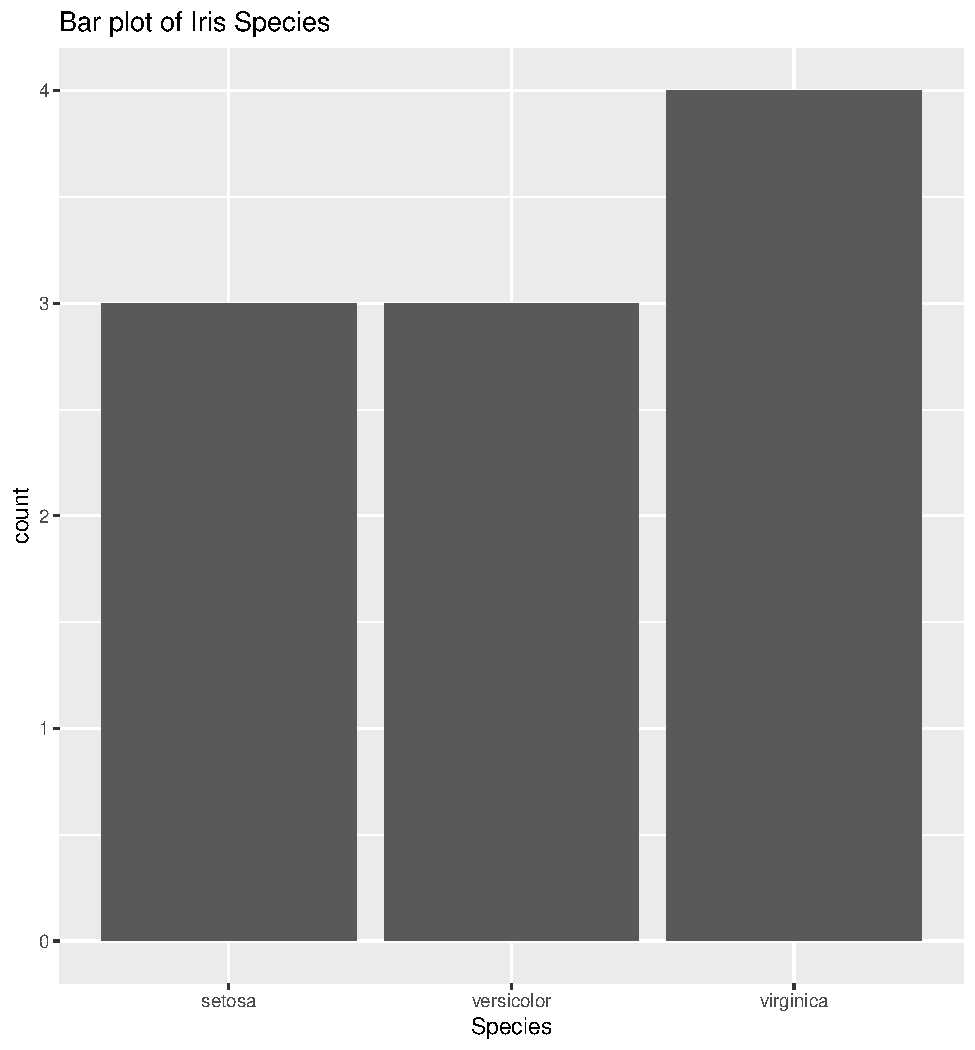
\includegraphics{_main_files/figure-latex/unnamed-chunk-4-1.pdf}

If needed (if you need proportions for the y-axis instead, calculate the
relative frequency table for the frequency table first). Note: again,
this one is missing the total

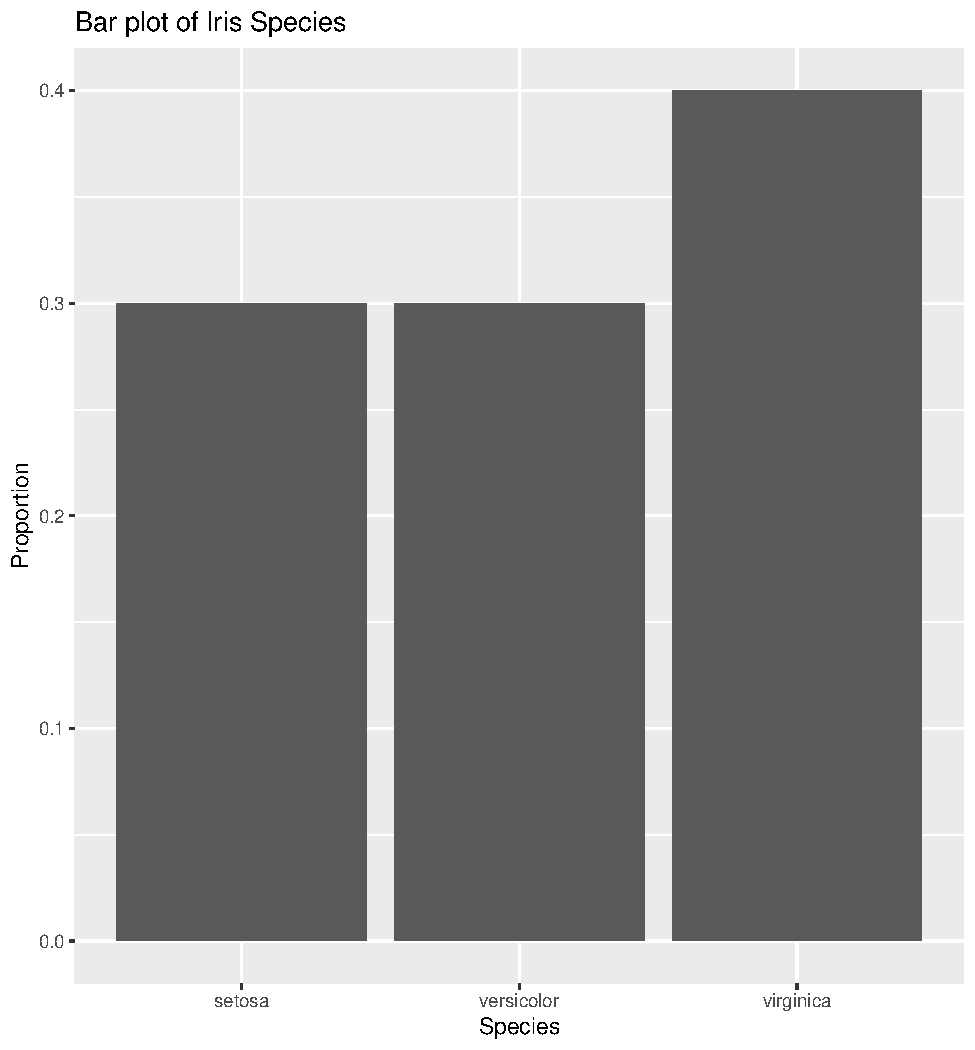
\includegraphics{_main_files/figure-latex/unnamed-chunk-6-1.pdf}

\hypertarget{stacked-bar-plots-and-side-by-side-bar-graphs}{%
\section{Stacked Bar Plots and Side-by-Side Bar Graphs}\label{stacked-bar-plots-and-side-by-side-bar-graphs}}

Stacked bar plots show two categorical variables, one on the
x-axis/y-axis, and the other as the legend (colours). We will call the
variable on the x-axis as the ``groups'' and the variable on the legend as
the ``categories.''

When constructing these bar plots, we first want to determine which
variable goes where (your choice or given choice to you). Then you
calculate relative frequencies \emph{per group}

For example, here I have a two-way table detailing the hair and eye
colour of some statistics students

\begin{verbatim}
## Warning: package 'reshape' was built under R version 4.1.3
\end{verbatim}

\begin{verbatim}
## 
## Attaching package: 'reshape'
\end{verbatim}

\begin{verbatim}
## The following object is masked from 'package:dplyr':
## 
##     rename
\end{verbatim}

\begin{verbatim}
## The following objects are masked from 'package:tidyr':
## 
##     expand, smiths
\end{verbatim}

So if I want eye colour to be my groups, I would calculate the relative
frequencies by column (use the total of the column and divide the whole
column by it), so each group/column will add up to 1.

These numbers will be my bar heights. So for the bar(s) representing
brown eyes:

\begin{itemize}
\item
  black hair will be .3091
\item
  brown hair will be .5409
\item
  red hair will be 0.1182
\item
  blond hair will be 0.0318
\end{itemize}

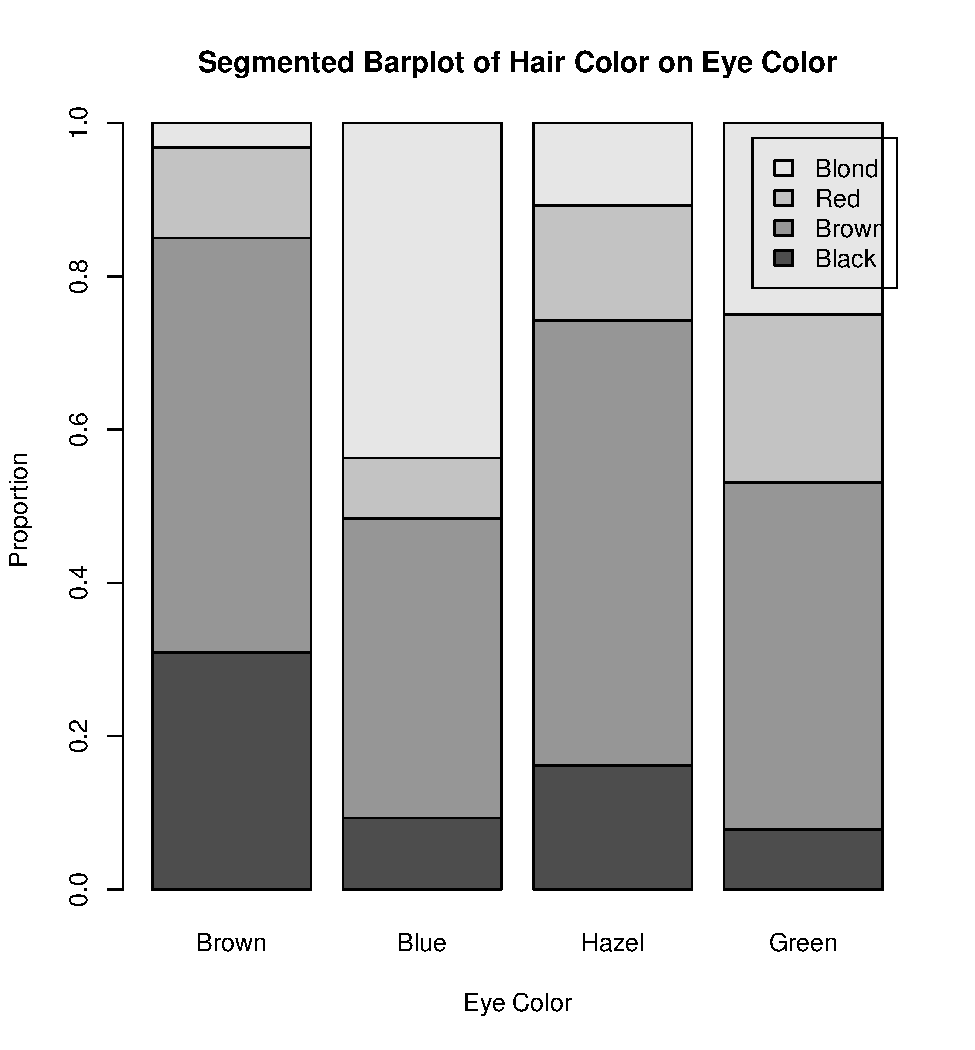
\includegraphics{_main_files/figure-latex/unnamed-chunk-9-1.pdf}

Here's the corresponding side-by-side bar plot. Note that the heights of
the bars are the same as the segmented bar graph.

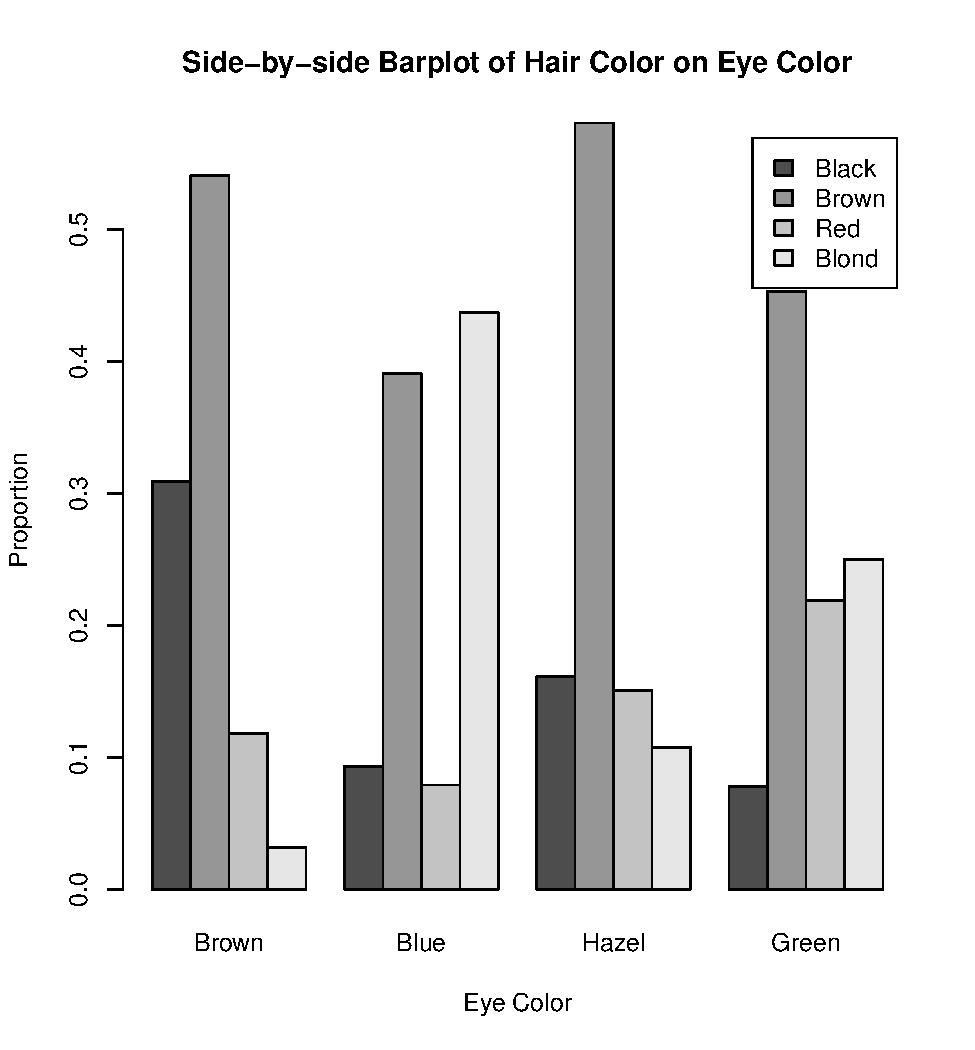
\includegraphics{_main_files/figure-latex/unnamed-chunk-10-1.pdf}

On the other hand, if I want my eye colour to be my groups, I would
calculate the relative frequencies by row (use the total of the row and
divide the whole row by it), so each group/row will add up to 1.

These numbers will be my bar heights. So for the bar(s) representing
black hair:

\begin{itemize}
\item
  brown eyes will be 0.6296296
\item
  blue eyes will be 0.1851852
\item
  hazel eyes will be 0.1388889
\item
  green eyes will be 0.0462963
\end{itemize}

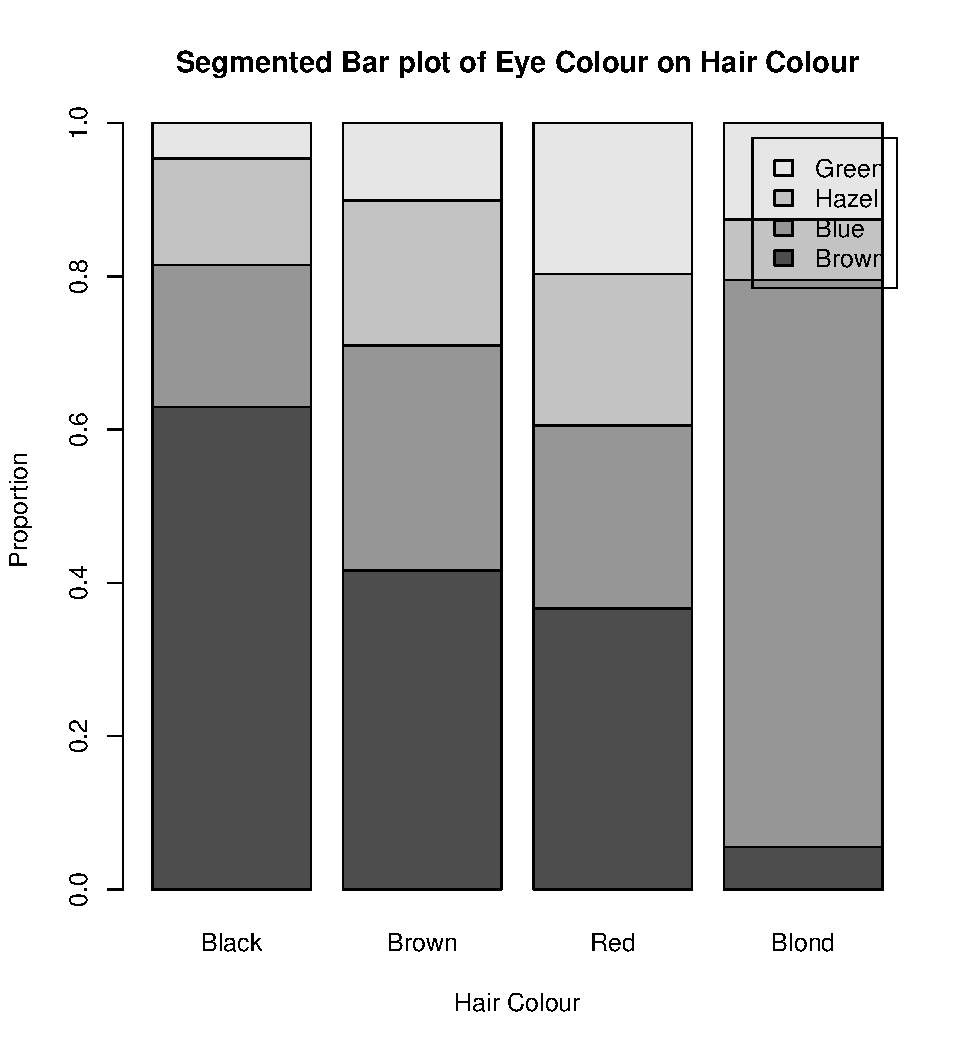
\includegraphics{_main_files/figure-latex/unnamed-chunk-12-1.pdf}

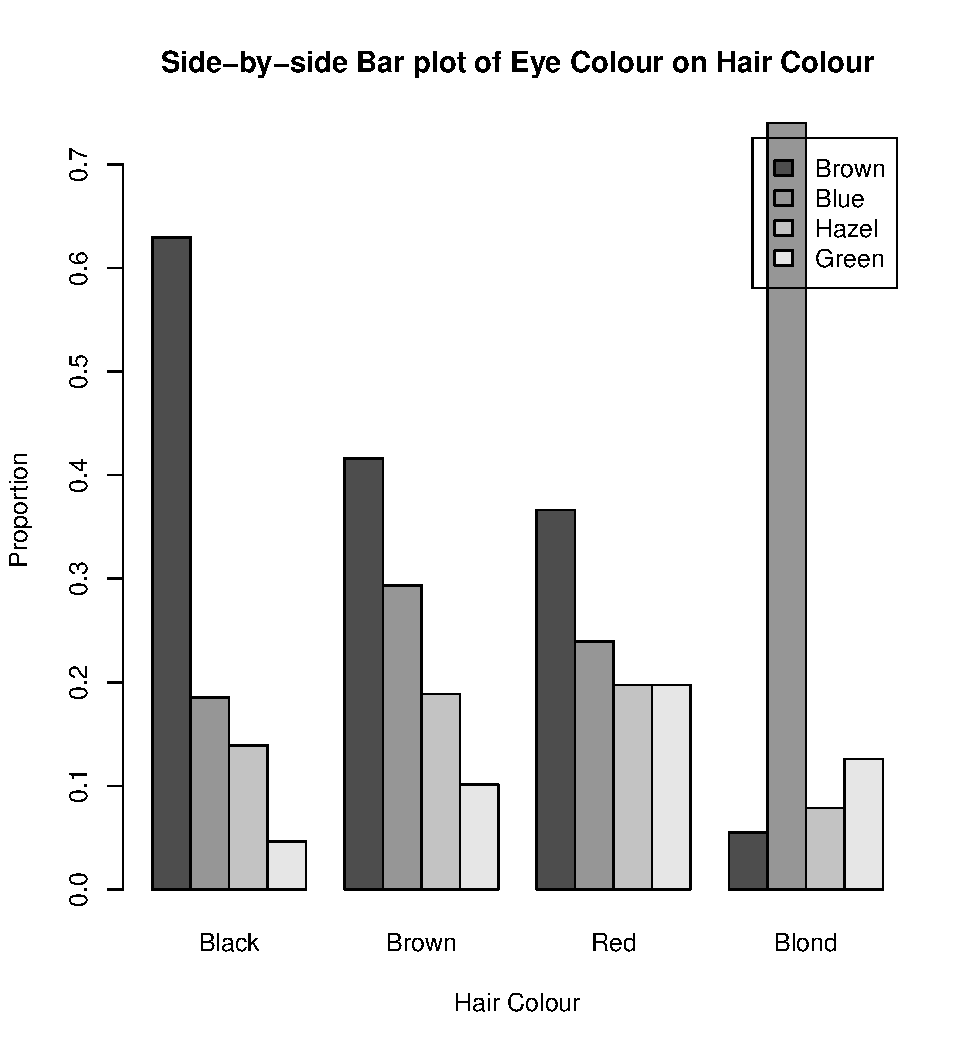
\includegraphics{_main_files/figure-latex/unnamed-chunk-13-1.pdf}

\hypertarget{mosaic-plots}{%
\section{Mosaic Plots}\label{mosaic-plots}}

Mosaic plots are the almost the same as stacked bar plots. The only
difference is that the widths of the bars change according to the
proportion of points in each group. In a mosaic plot, the x-axis will
also measure the proportion of observations/data points within the
groupings (i.e.~the x-axis reflects the marginal distribution of the
variable on the x-axis).

Following the \protect\hyperlink{stacked-bar-plots-and-side-by-side-bar-plots}{same
steps} as the
side-by-side and stacked bar charts to find the heights, we now add an
additional step before plotting.

\emph{Find the widths of the bars by finding the marginal distriubtion of the
variable on the x-axis (the groups)}

\begin{enumerate}
\def\labelenumi{\arabic{enumi}.}
\tightlist
\item
  For each group, find the probability of having that trait. So for
  our previous example, we had this table:
\end{enumerate}

Using our eye colours as the groups (vertical bars), we will find:

\begin{itemize}
\item
  \(P(Brown) \approx .3716\)
\item
  \(P(Blue) \approx .3632\)
\item
  \(P(Hazel) \approx .1571\)
\item
  \(P(Green) \approx .1081\)
\end{itemize}

When we plot our mosaic plot, we do the same thing, except now, we have
our bars differ in widths according to the numbers that we just
calculated.

\hypertarget{quantative-data-visualizations}{%
\chapter{Quantative Data Visualizations}\label{quantative-data-visualizations}}

\hypertarget{dot-plots}{%
\section{Dot Plots}\label{dot-plots}}

Dot plots are for discrete quantitative variables only, and they are
only useful in situations when you have a small range of number so that
you can actually see how the data distribution varies across values.

Dot plots are simple, you draw a number line and then plot points above
the number for each of the number that you see in the data.

Take this data for example:

Now count up each value to figure out how many dots you need at each
value on the number line then plot your graph

\begin{verbatim}
## Bin width defaults to 1/30 of the range of the data. Pick better value with `binwidth`.
\end{verbatim}

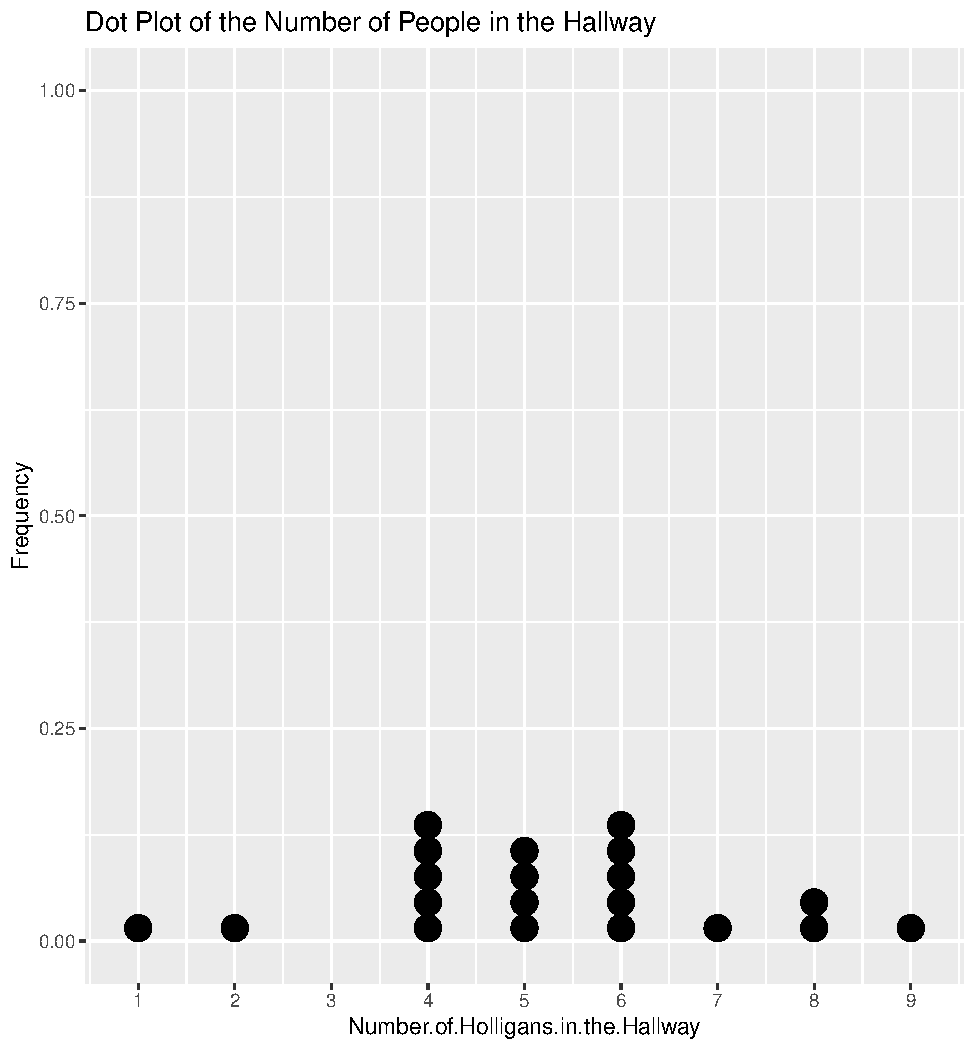
\includegraphics{_main_files/figure-latex/unnamed-chunk-16-1.pdf}

\hypertarget{stemplots}{%
\section{Stemplots}\label{stemplots}}

Using this data as an example, a stem plot looks like this:

A stem plot looks like this:

\begin{verbatim}
## 1 | 2: represents 12
##  leaf unit: 1
##             n: 20
##     0 | 1
##     1 | 8
##     2 | 
##     3 | 36689
##     4 | 4
##     5 | 2339
##     6 | 0228
##     7 | 
##     8 | 19
##     9 | 35
\end{verbatim}

In a stem plot, you need to determine a common ``stem'' of all the numbers
that you're plotting. So if you have integer numbers from 10 to 200,
your stems will be everything from the tens and so on, so you'll have
stems from 1-20. Once you take the stems, you just write the ``leaves''
next to the stem that they belong.

Note that you also have to add a key to show what a stem + leaf means.
The stem and leaves give no information on the decimals in the data, so
as you see above, you need to give an example like (as shown in the
example stemplot):

Key: 1\textbar2 = 12

Here's another example (sorted for convenience)

\begin{verbatim}
## 1 | 2: represents 1.2
##  leaf unit: 0.1
##             n: 50
##    3 | 3
##    3 | 579999
##    4 | 00334
##    4 | 556677788899
##    5 | 00112233444
##    5 | 667888999
##    6 | 234
##    6 | 5
##    7 | 12
\end{verbatim}

\hypertarget{boxplots}{%
\section{Boxplots}\label{boxplots}}

\emph{Also known as a box-and-whisker plot}

Boxplots are primarily made of the \textbf{five number summary} of the data.
The five number summary is made up of the:

\begin{itemize}
\item
  Minimum (min)
\item
  First Quartile (\(Q_1\))
\item
  Median
\item
  Third Quartile (\(Q_3\))
\item
  Maximum (max)
\end{itemize}

To make a simple boxplot, you use the first quartile, median, and third
quartile to make the ``box'' and then use the minimum and maximum to make
the ``whiskers.''

For this simple list of numbers:

Our five number summary is:

\begin{verbatim}
##    Min. 1st Qu.  Median 3rd Qu.    Max. 
##       1       2       4       6       7
\end{verbatim}

As detailed above, our box plot then looks like:

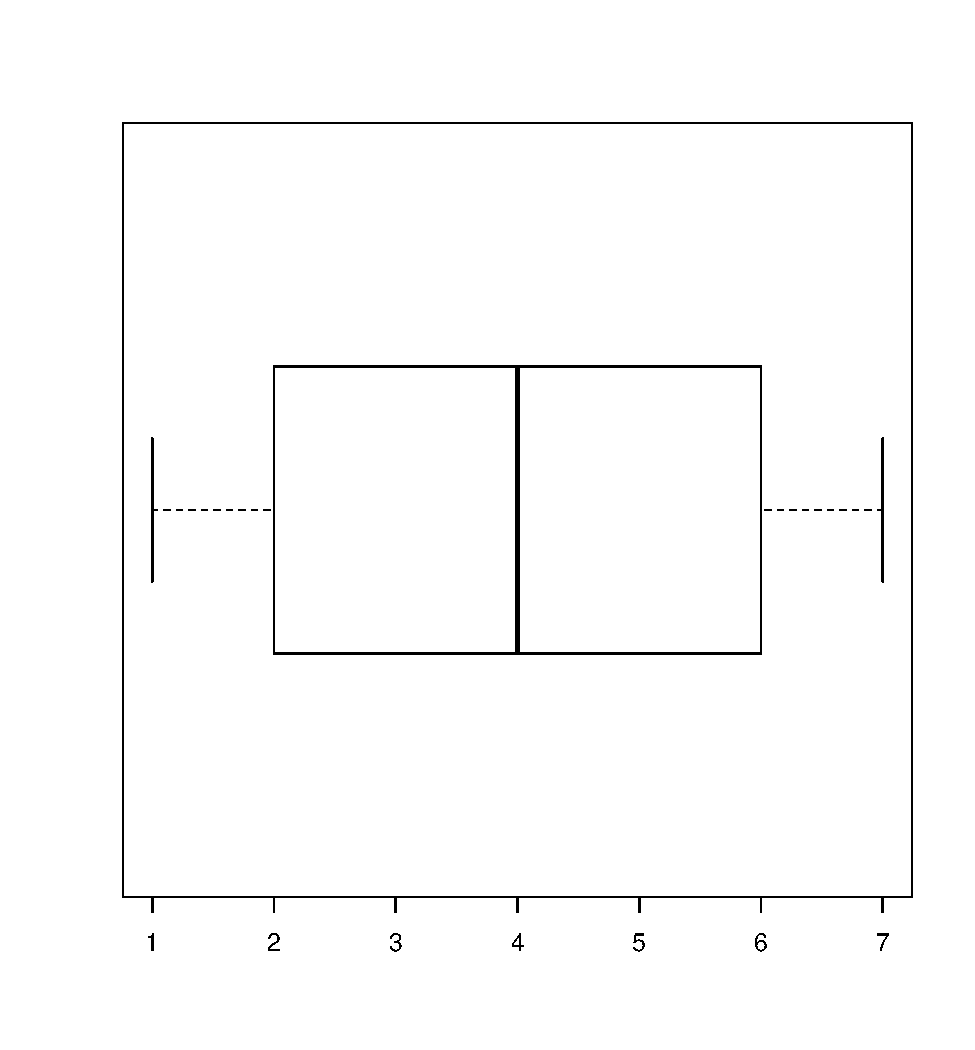
\includegraphics{_main_files/figure-latex/unnamed-chunk-22-1.pdf}

The last detail is that we can calculate outliers using the 1.5 IQR rule
and show them on the boxplot. For either direction (left or right), if
we see outliers in that direction, we only extend the whisker to the
smallest and/or largest point that is not an outlier. Then we plot any
outliers as individual points.

Look at this example data:

Five number summary:

\begin{verbatim}
##    Min. 1st Qu.  Median 3rd Qu.    Max. 
##     -12      -5      -3       0      12
\end{verbatim}

Our numbers calculated by the 1.5 IQR rule are:

\begin{verbatim}
## [1] -12.5   7.5
\end{verbatim}

So our 12 is an outlier. which means we draw our right whisker to 6 and
plot the 12 individually on the number line. Like so:

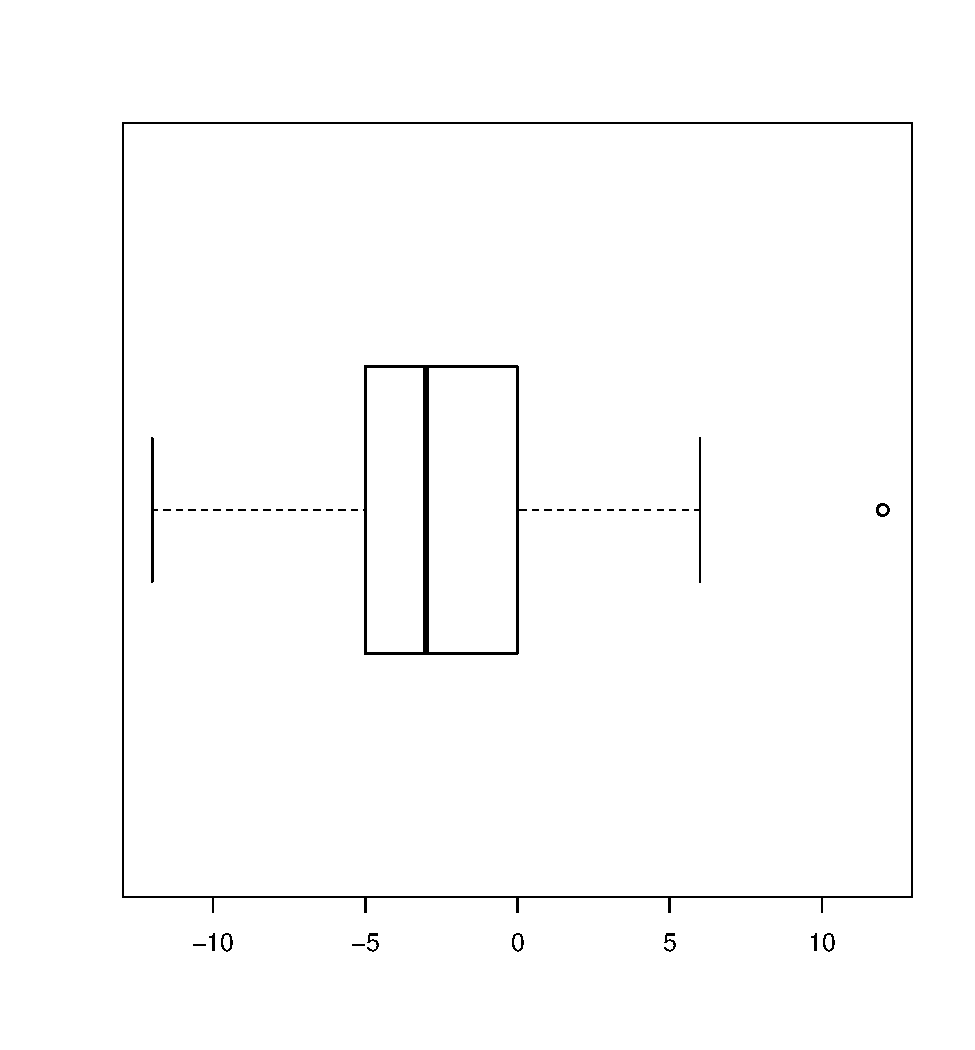
\includegraphics{_main_files/figure-latex/unnamed-chunk-26-1.pdf}

\hypertarget{histograms}{%
\section{Histograms}\label{histograms}}

A histogram is similar to a \protect\hyperlink{bar-plots}{bar plot}, except that
histograms are made for quantitative data and \emph{bars are continuous} in
the sense that there is no gap between bars. To make a histogram, select
an appropriate equal intervals that make it so that you don't have too
many bars and that you don't have too few bars. Your goal with
histograms, as with many other visualizations, is to be able to see the
shape and characteristics of the distribution in question. If you have
too many bars or too few bars, you won't be able to see much important
information (especially think of situations when you have many data
points with very precise decimal measurements).

\begin{enumerate}
\def\labelenumi{\arabic{enumi}.}
\item
  Decide on your intervals (e.g.~by 5's, by 10's, by 100's)
\item
  Within your intervals, count up the number of observations that
  belong in that ``bin''. When you do so, count up observations so that
  you count the left end inclusive and the right end inclusive. So if
  you did intervals of 5, you would do something like counting up
  points \(0 \leq x < 5\), \(5 \leq x < 10\), and so on.
\item
  Plot your bars.
\end{enumerate}

Example:

Consider this example data set:

Our data has this set of summary statistics:

\begin{verbatim}
##        x        
##  Min.   :1.522  
##  1st Qu.:1.912  
##  Median :2.022  
##  Mean   :2.110  
##  3rd Qu.:2.224  
##  Max.   :2.704
\end{verbatim}

With this knowledge, let's make our 7 ``bins'', so let's do these by every
0.2, starting at 1.5 to 2.9. This will be something that you build by
intuition.

Now, count up our values:

\begin{verbatim}
## [1.5,1.7) [1.7,1.9) [1.9,2.1) [2.1,2.3) [2.3,2.5) [2.5,2.7) [2.7,2.9] 
##         1         4         6         5         1         2         1
\end{verbatim}

Now, we just put it together. For each bin, we have a bar and the bars'
heights correspond to the number of individuals in each bin.

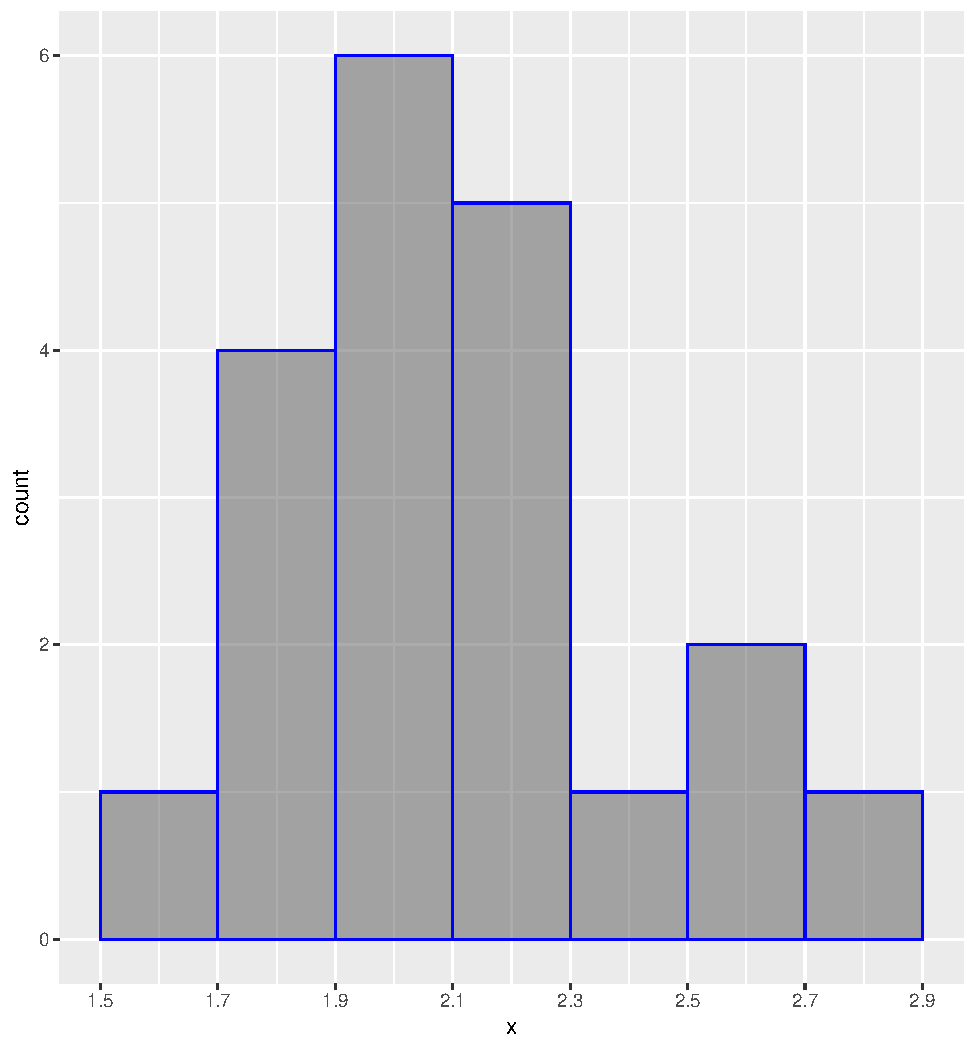
\includegraphics{_main_files/figure-latex/unnamed-chunk-30-1.pdf}

Again, just like bar graphs, we can instead do the relative frequencies
(this is what you'll see most of the time!!!)

\begin{verbatim}
## [1.5,1.7) [1.7,1.9) [1.9,2.1) [2.1,2.3) [2.3,2.5) [2.5,2.7) [2.7,2.9] 
##      0.05      0.20      0.30      0.25      0.05      0.10      0.05
\end{verbatim}

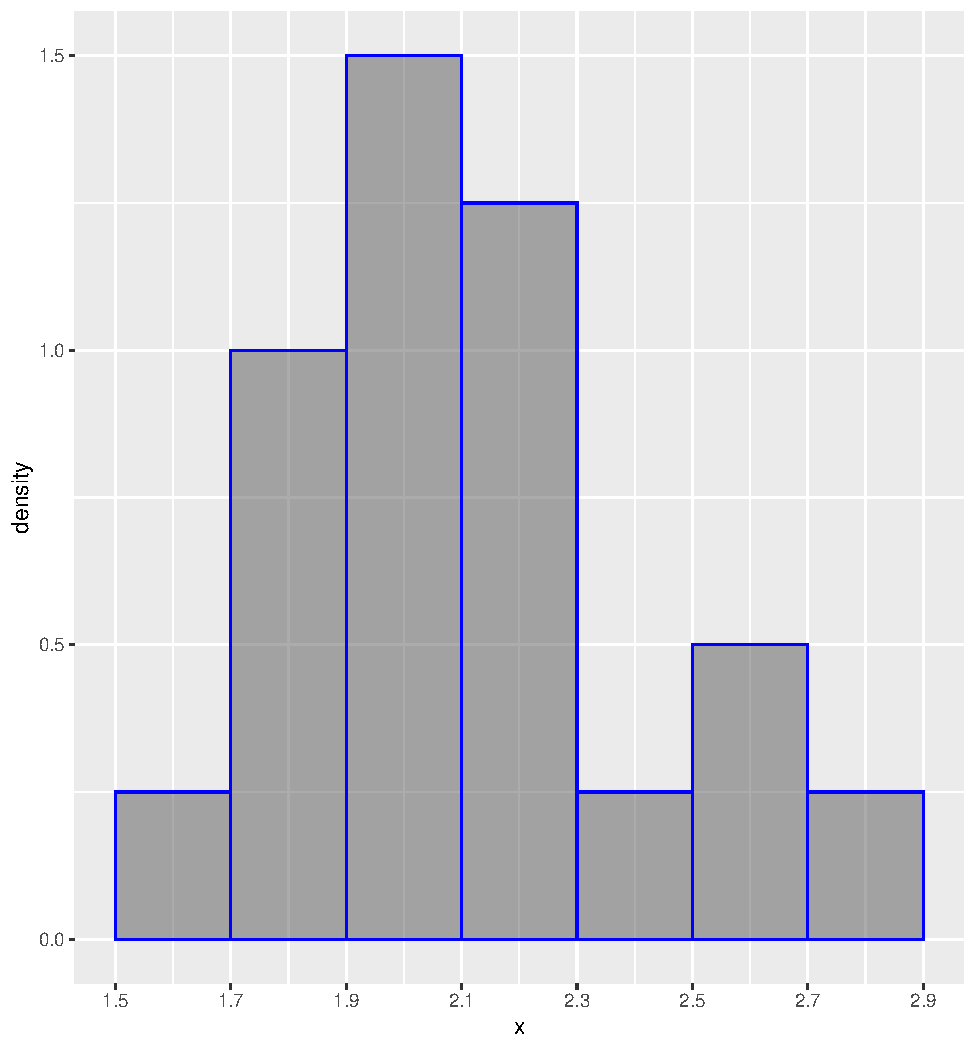
\includegraphics{_main_files/figure-latex/unnamed-chunk-32-1.pdf}

When you have a histogram like this, keep in mind that the bars always
add up to 1 (or 100\%).

\begin{center}\rule{0.5\linewidth}{0.5pt}\end{center}

\hypertarget{sampling}{%
\chapter{Sampling}\label{sampling}}

When we have a question about a certain population~(an entire group of
individuals). Ideally we would ask them all (take a \textbf{census}). But
contacting every member of a population often isn't very practical: it
would take too much time and cost too much money. Instead, we put the
question to a \textbf{sample}, or subset of individuals of the population
from which we actually collect data, chosen to represent the entire
population.

When you want to identify the population, ask yourself, what does the
question want to know about? What group of people does the
question/problem address?

When identifying the sample, ask yourself, what group does the work done
actually address?

\hypertarget{bias}{%
\section{Bias}\label{bias}}

When we collect data, there is the possibility of the data becoming
systematically pushed towards a specific outcome. For example, if we
want to learn about the GPA average in the school and take a sample of
students only from a class, it's quite possible that the sample is not
representative of the school. We will probably result in a GPA average
that is higher or lower than the actual GPA average in the school. There
are several ways that this can happen. The main way that we learn are:

\hypertarget{response-bias}{%
\subsection{Response Bias}\label{response-bias}}

\hypertarget{non-response-bias}{%
\subsection{Non-response Bias}\label{non-response-bias}}

\hypertarget{voluntary-bias}{%
\subsection{Voluntary Bias}\label{voluntary-bias}}

\hypertarget{probability}{%
\chapter{Probability}\label{probability}}

A process has a valid probability model if and only if:

\begin{itemize}
\tightlist
\item
  Each outcome has a positive probability.
\item
  The sum of all outcomes' probabilities is equal to 1.
\end{itemize}

\hypertarget{random-variables}{%
\chapter{Random Variables}\label{random-variables}}

A \textbf{random variable} is a variable whose value is a numerical outcome
of a random phenomenon.

Random variables can be discrete or continuous. A \textbf{discrete random
variable} \(X\) has a countable, or smaller, number of possible outcomes,
while a \textbf{continuous random variable} \(X\) can take on an infinite
number (theoretically) of different values.

The \textbf{probability distribution} of a random variable \(X\) gives us all
possible values of \(X\), and their corresponding probabilities.
Probability distributions are typically given as tables, histograms
(with probability on the y-axis, instead of frequency), or density
curves (like the Normal curve).

\hypertarget{discrete-random-variables}{%
\section{Discrete Random Variables}\label{discrete-random-variables}}

A discrete random variable describes a process that only has specific,
predefined outcomes. For example, you can be finding the probability of
people having blue, brown, and black eyes. Or you can be finding the
probability of people earning salaries in the ranges of \textless\$30,000,
\$30,000 - \$50,000, \$50,000 - \$ 70,000, \$70,000 - \$ 100,000,
\textgreater\$100,000.

When we have a discrete random variable \(X\) whose probability
distribution is

\[
\begin{aligned}
    \textbf{Value:}& ~~~~ x_1 ~~~~ x_2 ~~~~ x_3 ~~~~ \cdots \\
    \textbf{Probability:}& ~~~~ p_1 ~~~~ p_2 ~~~~ p_3 ~~~~\cdots
\end{aligned}
\]

we know the following about the mean and standard deviation of \(X\):

\[\mu_X = E(X) = \sum x_i P(x_i)\]

\[\sigma_X = \sqrt{\sum \left( x_i - \mu_X \right) ^2 P \left( x_i \right)}\]

Keep in mind that the standard deviation formula here (and else
where) is equivalent to the formula of population standard deviation
when we divide by \(n\) instead of multiplying by \(P(x_i)\).

\begin{align}
\sigma_X &= \sqrt{\frac{\sum(x_i - \mu_X)^2}{n}} \\
&=\sqrt{E((X - \bar x)^2)} \\
&=\sqrt{\sum \left( x_i - \mu_X \right) ^2 P \left( x_i \right)}\\
\end{align}

In other words, remember that we define standard deviation as the root
mean square of the squared differences from the mean. Since we are
taking the mean of the squared differences from the mean in both
formulas (I use the definition for mean from step 1 to 2 and the
definition of mean for discrete variables from step 2 to 3), the two
formulas are equivalent.

The variance of a random variable \(X\) is:

\[
Var(X) = \sigma_X^2
\]

\hypertarget{binomial-random-variables}{%
\subsection{Binomial Random Variables}\label{binomial-random-variables}}

Binomial random variables have parameters \(n\) and \(p\), and can be
written \(B(n, p)\). Remember, Normal random variables have parameters and
and can be written \(N(\mu,\sigma)\).

The pdf of a Binomial Random Variable (i.e.~the binomial formula) is:

\[
\begin{aligned}
    P(X=k) &= {n \choose k} p^k (1-p)^{n-k}\\
    \text{where } k &= 0, 1, 2, 3, \cdots, n
\end{aligned}
\]

To apply this formula in a graphing calculator:
\(\texttt{2nd -> vars (distr) -> binompdf}\)

Usage: \(\texttt{binompdf(n, p[,x])}\)

The cdf of a Binomial Random Variable is: \[
\begin{aligned}
    P(X\leq k) &= \sum_{i = 0}^n {n \choose i} p^i (1-p)^{n-i}
\end{aligned}
\]

In graphing calculator: \(\texttt{2nd -> vars (distr) -> binomcdf}\)

Usage: \(\texttt{binomcdf(n, p[,x])}\)

The mean and standard deviation of a binomial random variable is given
by:

\[
\begin{aligned}
    \mu_X &= n p \\
    \sigma_X &= \sqrt{n p q} \\
    &\text{, where } q = 1-p.
\end{aligned}
\]

\hypertarget{binomial-setting}{%
\subsubsection{Binomial setting}\label{binomial-setting}}

We can identify a binomial setting when we know:

\begin{enumerate}
\def\labelenumi{\arabic{enumi}.}
\item
  \textbf{B}inary? The possible outcomes of each trial can be classified as
  ``success'' or ``failure'' (in our case rolling a 7 or not).
\item
  \textbf{I}ndependent? Trials must be independent; that is, knowing the
  result of one trial must not tells us anything about the result of
  another trial.
\item
  \textbf{N}umber? The number of trials n of the chance process must be
  fixed in advance. (this was 5, then 100).
\item
  \textbf{S}ame? There is the same probability p of success on each trial
  (1/6).
\end{enumerate}

\hypertarget{condition}{%
\subsubsection{10\% Condition}\label{condition}}

The second condition is often not perfectly met, as in the case of an
SRS from some population. Imagine choosing 10 students from a class of
15 females and 15 males---as we choose people, the remaining population
changes, which changes the probability that the next person chosen will
be male or female.

When we lack complete independence, we can see the consequence of this
is negligible as long as our sample is small relative to the population
from which we are sampling. If we were choosing our 10 people from a
school of 3,300 students, the change in probability from person to
person would be small enough to ignore.

The general rule is that the sample needs to be less than
\(\frac{1}{10}\), or 10\%, of the population. We refer to this as the 10\%
condition.

\[n \leq (.10) N\]

\hypertarget{normal-approximation-to-the-binomial-distribution}{%
\subsubsection{Normal Approximation to the Binomial Distribution}\label{normal-approximation-to-the-binomial-distribution}}

Remember that as \(n\) gets large, a binomial random variable \(X\) can take
on more and more different values, and it can become tedious to continue
to treat X as a discrete random variable. As \(n\) get larger, we can
treat \(X\) as a continuous random variable, more specifically:

As \(n\) gets larger, the binomial distribution gets closer to a normal
distribution. However, before we use a normal distribution to
approximate a binomial distribution, we have to check the following
condition:

\hypertarget{large-counts-condition}{%
\paragraph{Large Counts condition}\label{large-counts-condition}}

If \(np \geq 10\) and \(n(1-p) \geq 10\), then we can use a Normal
distribution to model a binomial distribution. In other words, if the
expected number of successes and failures (respectively) is greater than
or equal to 10.

\hypertarget{doing-a-normal-approximation}{%
\paragraph{Doing a normal approximation}\label{doing-a-normal-approximation}}

First verify all the conditions for a Binomial setting and the Large
Counts Condition. Since we know that we have a binomial setting, we then
know the distribution that we want to use is \(Normal(np, \sqrt{npq})\) proceed with the calculations according to this distribution.

\hypertarget{geometric-random-variables}{%
\subsection{Geometric Random Variables}\label{geometric-random-variables}}

If \(X \sim G(p)\), in other words, if \(X\) has a geometric distribution
with parameter \(p\), the pdf of a geometric random variable is:

\[
\begin{aligned}
    P(X=x) &= (1-p)^{x-1}p\\
    \text{where } x &= 1, 2, 3, \cdots
\end{aligned}
\]

In graphing calculator: \(\texttt{2nd -> vars (distr) -> geometpdf}\)

Usage: \(\texttt{geometpdf(p, x)}\)

The cdf of a Geometric Variable is:

\[
\begin{aligned}
    P(X\leq x) &= \sum_{i=1}^x(1-p)^{i-1}p
\end{aligned}
\]

In graphing calculator: \(\texttt{2nd -> vars (distr) -> geometcdf}\)

Usage: \(\texttt{geometcdf(p, x)}\)

The mean and standard deviation of a geometric random variable is given
by:

\[
\begin{aligned}
    \mu_X &= \frac{1}{p} \\
    \sigma_X &= \frac{\sqrt{q}}{p} \\
    &\text{, where } q = 1-p.
\end{aligned}
\]

\hypertarget{the-geometric-setting}{%
\subsubsection{The Geometric Setting}\label{the-geometric-setting}}

A geometric setting is very similar to a binomial setting, except that
\textbf{n, the number of trials is not fixed}.

A geometric setting is defined as a series of observations where these 4
conditions are met:

\begin{enumerate}
\def\labelenumi{\arabic{enumi}.}
\item
  \textbf{B}inary? The Possible outcomes of each trial can be classified as
  ``success'' or ``failure''
\item
  \textbf{I}ndependent? Trials must be independent, that is, knowing the
  result of one trial must not have any effect on the result of any
  other trial.
\item
  \textbf{T}rials? The goal is to count the number of trials until the
  first success occurs.
\item
  \textbf{S}uccess? On each trial, the probability p of success must be the
  same.
\end{enumerate}

\hypertarget{operations-with-random-variables}{%
\section{Operations with Random Variables}\label{operations-with-random-variables}}

\hypertarget{constants}{%
\subsection{Constants}\label{constants}}

When we add a constant \(a\) and/or multiply by a constant \(b\) to a random
variable \(X\), we perform a linear transformation of the form

\[
a + bX
\]

The mean of the transformed variable is:

\[
\mu_{a+bX}=a+\mu_{bX}=a+b\mu_X
\]

The standard deviation of the transformed variable is:

\[
\sigma_{a+bX}=\sigma_{bX}=b\sigma_X
\]

\hypertarget{random-variables-1}{%
\subsection{Random Variables}\label{random-variables-1}}

In general, we can describe the mean and standard deviation of the sum
or difference of independent random variables with these formulas:

\[\mu_{X \pm Y} = \mu_X \pm \mu_Y\]

\textbf{If the random variables \(X\) and \(Y\) are independent}, then

\[ \sigma_{X \pm Y}^2 = \sigma_X^2 + \sigma_Y^2 \]

\hypertarget{hello-bookdown}{%
\chapter{Hello bookdown}\label{hello-bookdown}}

All chapters start with a first-level heading followed by your chapter title, like the line above. There should be only one first-level heading (\texttt{\#}) per .Rmd file.

\hypertarget{a-section}{%
\section{A section}\label{a-section}}

All chapter sections start with a second-level (\texttt{\#\#}) or higher heading followed by your section title, like the sections above and below here. You can have as many as you want within a chapter.

\hypertarget{an-unnumbered-section}{%
\subsection*{An unnumbered section}\label{an-unnumbered-section}}
\addcontentsline{toc}{subsection}{An unnumbered section}

Chapters and sections are numbered by default. To un-number a heading, add a \texttt{\{.unnumbered\}} or the shorter \texttt{\{-\}} at the end of the heading, like in this section.

\hypertarget{cross}{%
\chapter{Cross-references}\label{cross}}

Cross-references make it easier for your readers to find and link to elements in your book.

\hypertarget{chapters-and-sub-chapters}{%
\section{Chapters and sub-chapters}\label{chapters-and-sub-chapters}}

There are two steps to cross-reference any heading:

\begin{enumerate}
\def\labelenumi{\arabic{enumi}.}
\tightlist
\item
  Label the heading: \texttt{\#\ Hello\ world\ \{\#nice-label\}}.

  \begin{itemize}
  \tightlist
  \item
    Leave the label off if you like the automated heading generated based on your heading title: for example, \texttt{\#\ Hello\ world} = \texttt{\#\ Hello\ world\ \{\#hello-world\}}.
  \item
    To label an un-numbered heading, use: \texttt{\#\ Hello\ world\ \{-\#nice-label\}} or \texttt{\{\#\ Hello\ world\ .unnumbered\}}.
  \end{itemize}
\item
  Next, reference the labeled heading anywhere in the text using \texttt{\textbackslash{}@ref(nice-label)}; for example, please see Chapter \ref{cross}.

  \begin{itemize}
  \tightlist
  \item
    If you prefer text as the link instead of a numbered reference use: \protect\hyperlink{cross}{any text you want can go here}.
  \end{itemize}
\end{enumerate}

\hypertarget{captioned-figures-and-tables}{%
\section{Captioned figures and tables}\label{captioned-figures-and-tables}}

Figures and tables \emph{with captions} can also be cross-referenced from elsewhere in your book using \texttt{\textbackslash{}@ref(fig:chunk-label)} and \texttt{\textbackslash{}@ref(tab:chunk-label)}, respectively.

See Figure \ref{fig:nice-fig}.

\begin{figure}

{\centering 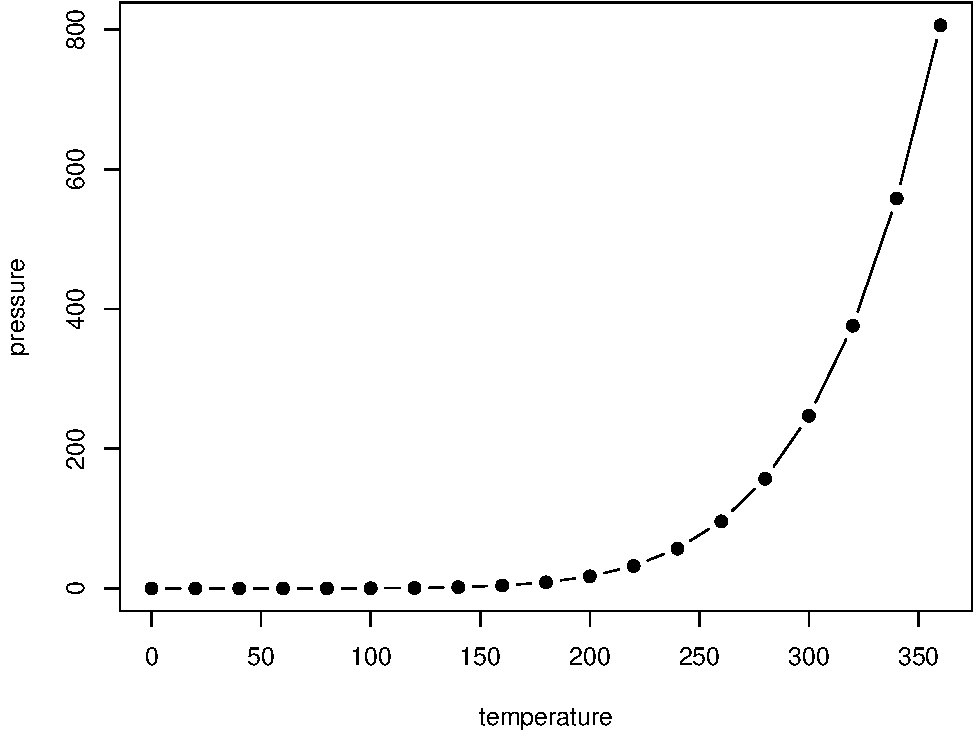
\includegraphics[width=0.8\linewidth]{_main_files/figure-latex/nice-fig-1} 

}

\caption{Here is a nice figure!}\label{fig:nice-fig}
\end{figure}

Don't miss Table \ref{tab:nice-tab}.

\begin{table}

\caption{\label{tab:nice-tab}Here is a nice table!}
\centering
\begin{tabular}[t]{rr}
\toprule
temperature & pressure\\
\midrule
0 & 0.0002\\
20 & 0.0012\\
40 & 0.0060\\
60 & 0.0300\\
80 & 0.0900\\
\addlinespace
100 & 0.2700\\
120 & 0.7500\\
140 & 1.8500\\
160 & 4.2000\\
180 & 8.8000\\
\bottomrule
\end{tabular}
\end{table}

\hypertarget{parts}{%
\chapter{Parts}\label{parts}}

You can add parts to organize one or more book chapters together. Parts can be inserted at the top of an .Rmd file, before the first-level chapter heading in that same file.

Add a numbered part: \texttt{\#\ (PART)\ Act\ one\ \{-\}} (followed by \texttt{\#\ A\ chapter})

Add an unnumbered part: \texttt{\#\ (PART\textbackslash{}*)\ Act\ one\ \{-\}} (followed by \texttt{\#\ A\ chapter})

Add an appendix as a special kind of un-numbered part: \texttt{\#\ (APPENDIX)\ Other\ stuff\ \{-\}} (followed by \texttt{\#\ A\ chapter}). Chapters in an appendix are prepended with letters instead of numbers.

\hypertarget{footnotes-and-citations}{%
\chapter{Footnotes and citations}\label{footnotes-and-citations}}

\hypertarget{footnotes}{%
\section{Footnotes}\label{footnotes}}

Footnotes are put inside the square brackets after a caret \texttt{\^{}{[}{]}}. Like this one \footnote{This is a footnote.}.

\hypertarget{citations}{%
\section{Citations}\label{citations}}

Reference items in your bibliography file(s) using \texttt{@key}.

For example, we are using the \textbf{bookdown} package \citep{R-bookdown} (check out the last code chunk in index.Rmd to see how this citation key was added) in this sample book, which was built on top of R Markdown and \textbf{knitr} \citep{xie2015} (this citation was added manually in an external file book.bib).
Note that the \texttt{.bib} files need to be listed in the index.Rmd with the YAML \texttt{bibliography} key.

The RStudio Visual Markdown Editor can also make it easier to insert citations: \url{https://rstudio.github.io/visual-markdown-editing/\#/citations}

\hypertarget{blocks}{%
\chapter{Blocks}\label{blocks}}

\hypertarget{equations}{%
\section{Equations}\label{equations}}

Here is an equation.

\begin{equation} 
  f\left(k\right) = \binom{n}{k} p^k\left(1-p\right)^{n-k}
  \label{eq:binom}
\end{equation}

You may refer to using \texttt{\textbackslash{}@ref(eq:binom)}, like see Equation \eqref{eq:binom}.

\hypertarget{theorems-and-proofs}{%
\section{Theorems and proofs}\label{theorems-and-proofs}}

Labeled theorems can be referenced in text using \texttt{\textbackslash{}@ref(thm:tri)}, for example, check out this smart theorem \ref{thm:tri}.

\begin{theorem}
\protect\hypertarget{thm:tri}{}\label{thm:tri}For a right triangle, if \(c\) denotes the \emph{length} of the hypotenuse
and \(a\) and \(b\) denote the lengths of the \textbf{other} two sides, we have
\[a^2 + b^2 = c^2\]
\end{theorem}

Read more here \url{https://bookdown.org/yihui/bookdown/markdown-extensions-by-bookdown.html}.

\hypertarget{callout-blocks}{%
\section{Callout blocks}\label{callout-blocks}}

The R Markdown Cookbook provides more help on how to use custom blocks to design your own callouts: \url{https://bookdown.org/yihui/rmarkdown-cookbook/custom-blocks.html}

\hypertarget{sharing-your-book}{%
\chapter{Sharing your book}\label{sharing-your-book}}

\hypertarget{publishing}{%
\section{Publishing}\label{publishing}}

HTML books can be published online, see: \url{https://bookdown.org/yihui/bookdown/publishing.html}

\hypertarget{pages}{%
\section{404 pages}\label{pages}}

By default, users will be directed to a 404 page if they try to access a webpage that cannot be found. If you'd like to customize your 404 page instead of using the default, you may add either a \texttt{\_404.Rmd} or \texttt{\_404.md} file to your project root and use code and/or Markdown syntax.

\hypertarget{metadata-for-sharing}{%
\section{Metadata for sharing}\label{metadata-for-sharing}}

Bookdown HTML books will provide HTML metadata for social sharing on platforms like Twitter, Facebook, and LinkedIn, using information you provide in the \texttt{index.Rmd} YAML. To setup, set the \texttt{url} for your book and the path to your \texttt{cover-image} file. Your book's \texttt{title} and \texttt{description} are also used.

This \texttt{gitbook} uses the same social sharing data across all chapters in your book- all links shared will look the same.

Specify your book's source repository on GitHub using the \texttt{edit} key under the configuration options in the \texttt{\_output.yml} file, which allows users to suggest an edit by linking to a chapter's source file.

Read more about the features of this output format here:

\url{https://pkgs.rstudio.com/bookdown/reference/gitbook.html}

Or use:

  \bibliography{book.bib,packages.bib}

\end{document}
